\documentclass[10pt,xcolor={usenames,dvipsnames}]{beamer}
% \documentclass{bredelebeamer}
\usetheme{JuanLesPins}

\usepackage[T2A]{fontenc}
\usepackage[utf8]{inputenc}
\usepackage{color}
\usepackage{graphicx}
\usepackage{listings}
\usepackage{lmodern}



\lstset{
	frame=tb, % draw a frame at the top and bottom of the code block
	tabsize=4, % tab space width
	showstringspaces=false, % don't mark spaces in strings
	numbers=left, % display line numbers on the left
	commentstyle=\color{green}, % comment color
	keywordstyle=\color{blue}, % keyword color
	stringstyle=\color{red},% string color
	basicstyle=\tiny
}

% \graphicspath{/media/sf\_work/docs/presentations/memory/img}
\graphicspath{{Figures/}{img/}}

% TODO: default, destructor with delete, output addres
%
%
%
\begin{document}

\title{Design Patterns}
\author{Denis Ponizovkin} 

\institute[<EPAM>]

\frame{\titlepage} 

\section{Introduction}
\begin{frame}[fragile]
	\frametitle{Design Pattern}
	\begin{exampleblock}{Definition}
	In software engineering, a software design pattern is a general,
	reusable solution to a commonly occurring problem within a given
	context in software design.
	\end{exampleblock}
\end{frame}

\begin{frame}[fragile]
	\frametitle{Roots}
	\begin{exampleblock}{}
		The idea was introduced by the architect Christopher Alexander
		and has been adapted for various other disciplines, most notably
		computer science.
	\end{exampleblock}

	\begin{exampleblock}{}
	\begin{quote}
The elements of this language are entities called patterns. Each pattern describes a problem that occurs over and over again in our environment, and then describes the core of the solution to that problem, in such a way that you can use this solution a million times over, without ever doing it the same way twice. --- Christopher Alexander
	\end{quote}
	\end{exampleblock}
\end{frame}

\begin{frame}[fragile]
	\frametitle{From architecture to software}
	\begin{exampleblock}{GoF}
	\begin{quote}
Christopher Alexander is the architect who first studied patterns in buildings and communications and developed "pattern language" for generating them. His work has inspired us time and again. There are many ways in which our work is like Alexander's. Both are based on observing existing systems and looking for patterns in them. Both have templates for describing patterns. Both rely on natural language and lots of examples to described patterns rather than formal languages, and both give rationales for each pattern. --- Design Patterns.
	\end{quote}
	\end{exampleblock}
\end{frame}

\begin{frame}[fragile]
	\frametitle{Why do I need to study patterns}
	\begin{itemize}
		\item Reusability;
		\item The use of common terminology;
		\item Design patterns provide us with an abstract, high-level view of
		both the problem and the whole process of object-oriented development.
	\item design patterns allow a developer or a group of developers to find design solutions for complex problems without creating a cumbersome class inheritance hierarchy.
	\end{itemize}
\end{frame}

\begin{frame}[fragile]
	\frametitle{Other advantages}
	\begin{itemize}
		\item Efficiency improvement of single developers and whole group of developers;
		\item The use of many design patterns also allows you to create more modifiable and flexible software;
		\item Properly studied design patterns greatly assist in a common understanding of the basic principles of object-oriented design. 
	\end{itemize}
\end{frame}

\section{UML reminder}
\subsection{Association}
\begin{frame}[fragile]
	\frametitle{Association}
	\begin{exampleblock}{}
	If two classes in a model need to communicate with each other, there must be link between them, and that can be represented by an association (connector).
	We can define a one-to-one, one-to-many, many-to-one and many-to-many relationship among objects.
	\end{exampleblock}

	\begin{figure}
		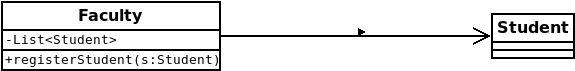
\includegraphics[height=1.5cm,width=8cm]{unidir-association.png}
		\caption{Unidirectional assocation example}
	\end{figure}

	\begin{figure}
		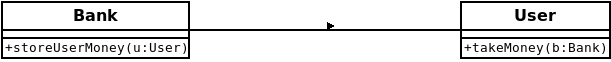
\includegraphics[height=1.5cm,width=8cm]{bidir-association.png}
		\caption{Bidirectional assocation example}
	\end{figure}
\end{frame}

\subsection{Aggregation}
\begin{frame}[fragile]
	\frametitle{Aggregation}
		\begin{figure}
			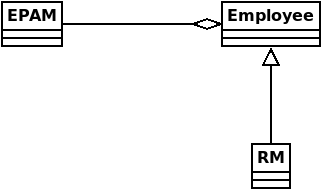
\includegraphics[height=5cm,width=6cm]{aggregation.png}
		\end{figure}
\end{frame}

\subsection{Composition}
\begin{frame}[fragile]
	\frametitle{Composition}
		\begin{figure}
			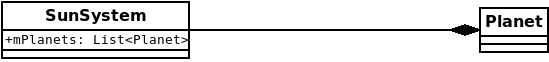
\includegraphics[height=2cm,width=8cm]{composition.png}
		\end{figure}
\end{frame}

\subsection{Association, aggregation, composition}
\begin{frame}[fragile]
	\frametitle{Association, aggregation, composition}
		\begin{figure}
			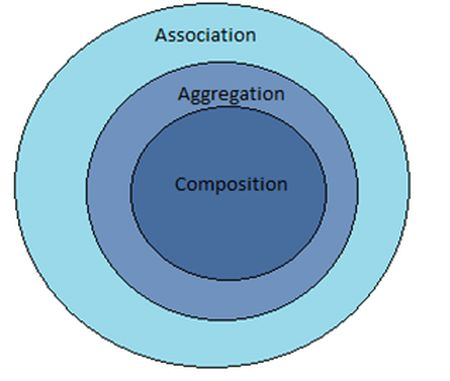
\includegraphics[height=5cm,width=6cm]{aac.jpg}
		\end{figure}
\end{frame}

\section{Structural Patterns}
\begin{frame}[fragile]
	\frametitle{Definition}
	\begin{exampleblock}{}
	Structural patterns are concerned with how classes and objects are composed to form
	larger structures. Structural class patterns use inheritance to compose interfaces or
	implementations. Structural object patterns describe ways to compose objects to
	realize new functionality.
	\end{exampleblock}
\end{frame}

\subsection{Facade}
\begin{frame}[fragile]
	\frametitle{Intent}
	\begin{exampleblock}{}
	Provide a unified interface to a set of interfaces in a subsystem. Facade defines a
	higher-level interface that makes the subsystem easier to use.
	\end{exampleblock}
\end{frame}

\begin{frame}[fragile]
	\frametitle{Motivation}
	\begin{exampleblock}{}
Structuring a system into subsystems helps reduce complexity. A common design goal is to minimize the communication and dependencies between subsystems. One way to achieve this goal is to introduce a facade object that provides a single, simplified interface to the more general facilities of a subsystem.
	\end{exampleblock}
\end{frame}

\begin{frame}[fragile]
	\frametitle{Example}
		\begin{figure}
			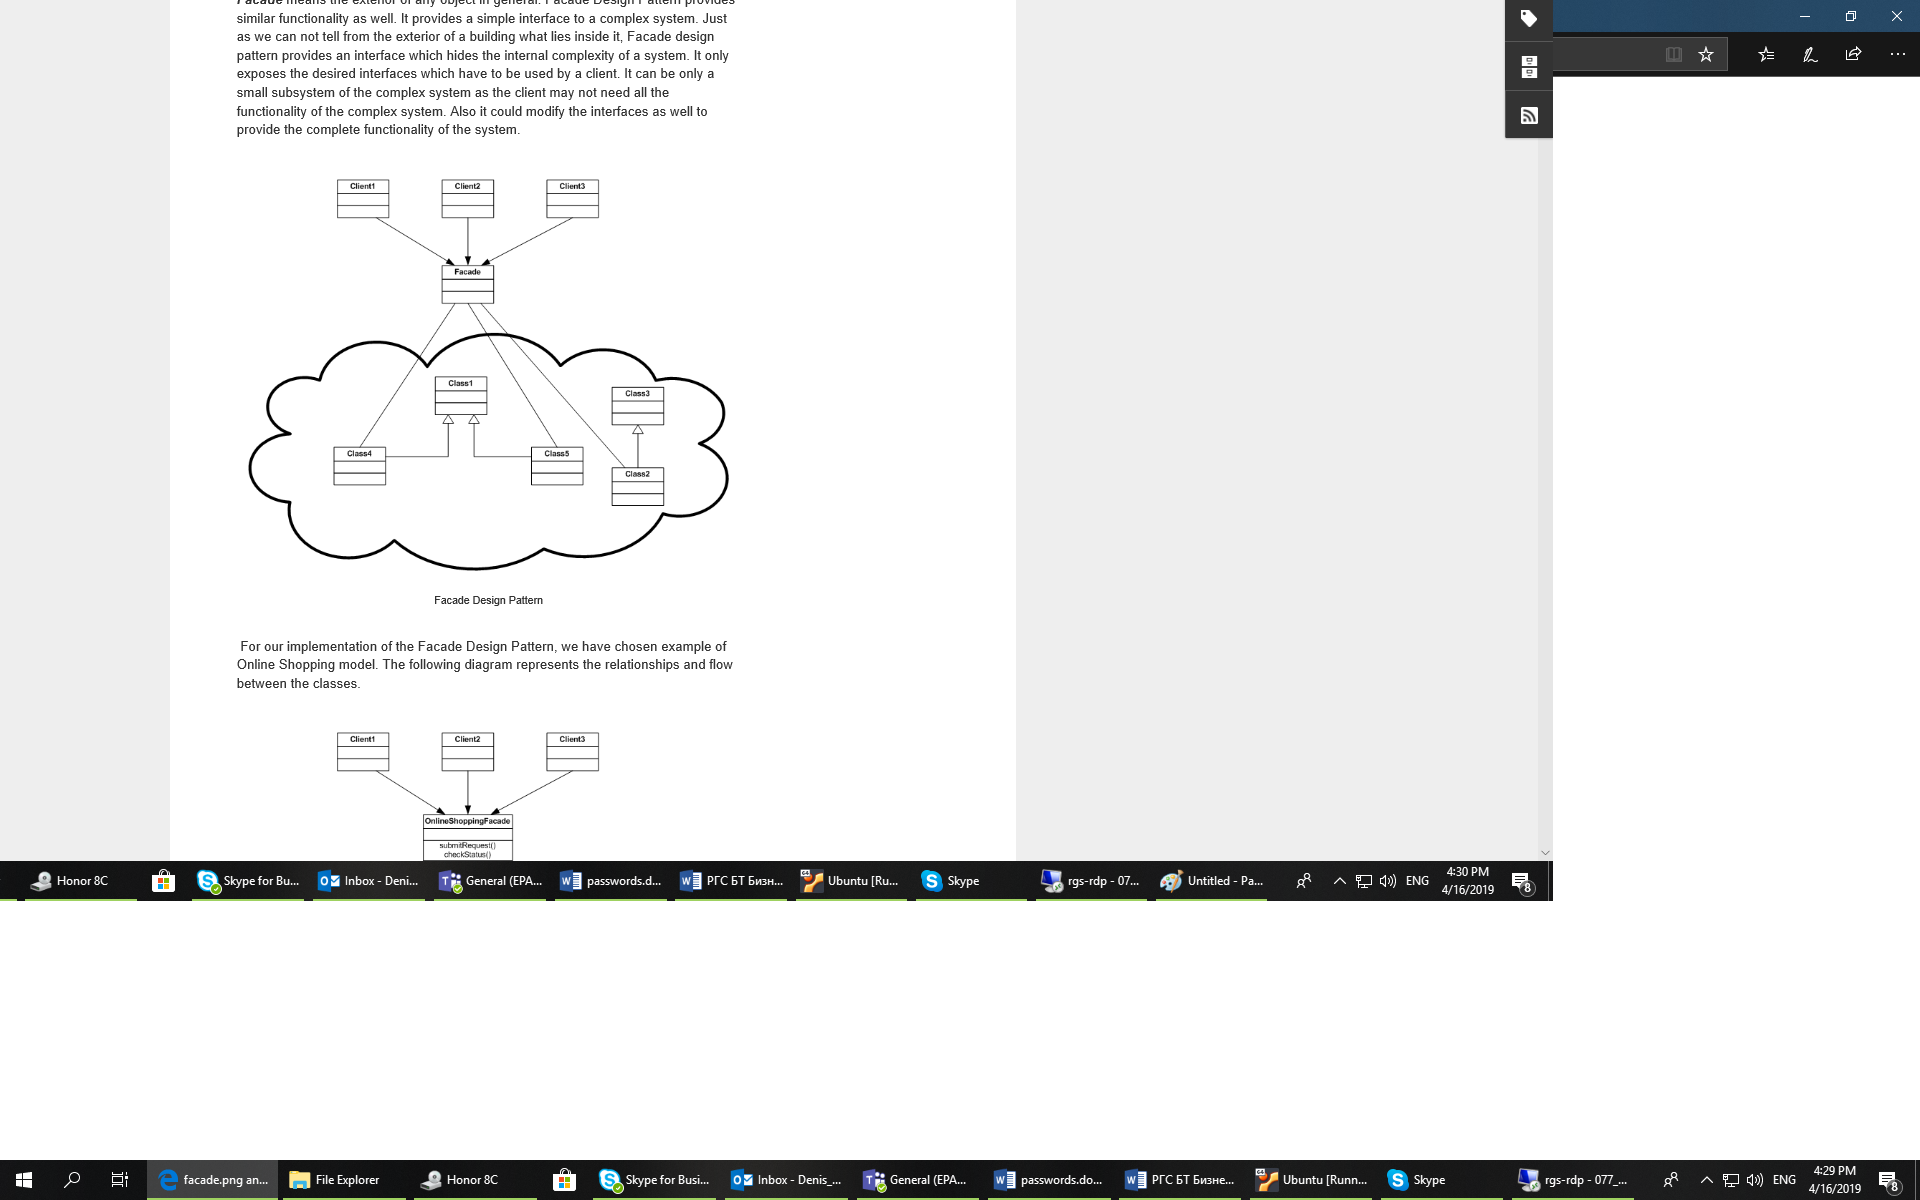
\includegraphics[height=7cm,width=8cm]{facade.png}
			\caption{Facade for starting a car system}
		\end{figure}
\end{frame}

\begin{frame}[fragile]
	\frametitle{Applicability}
	\begin{exampleblock}{}
		\begin{itemize}
			\item you want to provide a simple interface to a complex subsystem;
			\item there are many dependencies between clients and the implementation classes
of an abstraction;
			\item you want to layer your subsystems.
		\end{itemize}
	\end{exampleblock}
\end{frame}

\subsection{Adapter (wrapper)}
\begin{frame}[fragile]
	\frametitle{Intent}
	\begin{exampleblock}{}
	Convert the interface of a class into another interface clients expect. Adapter lets
	classes work together that couldn't otherwise because of incompatible interfaces.
	\end{exampleblock}
\end{frame}

\begin{frame}[fragile]
	\frametitle{Motivation}
	\begin{exampleblock}{}
	Sometimes a toolkit class that's designed for reuse isn't reusable only because its
	interface doesn't match the domain-specific interface an application requires.
	\end{exampleblock}
\end{frame}

\begin{frame}[fragile]
	\frametitle{Example. The task}
	\begin{figure}
		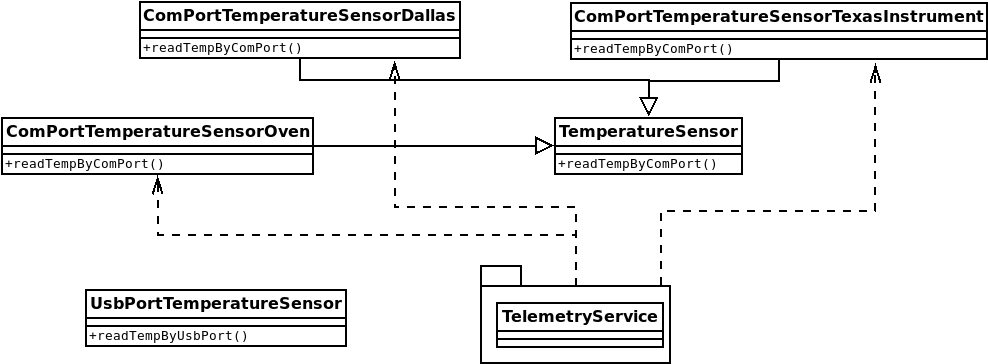
\includegraphics[height=4cm,width=8cm]{adapter-task.png}
		\caption{Adapter usage case}
	\end{figure}
\end{frame}

\begin{frame}[fragile]
	\frametitle{Example. The task resolution}
	\begin{figure}
		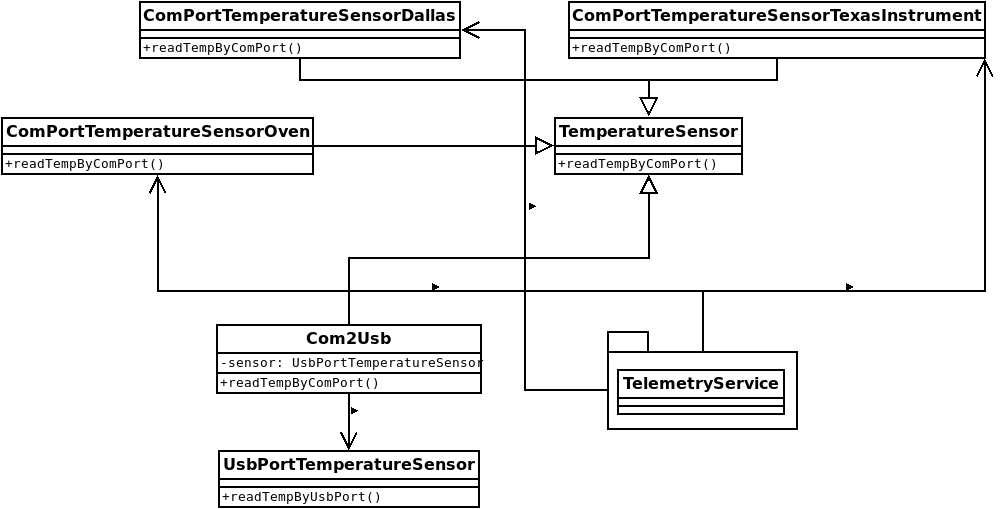
\includegraphics[height=4cm,width=8cm]{adapter-task-resolution1.png}
		\caption{Adapter usage case}
	\end{figure}
\end{frame}

\begin{frame}[fragile]
	\frametitle{Example. The task resolution}
	\begin{figure}
		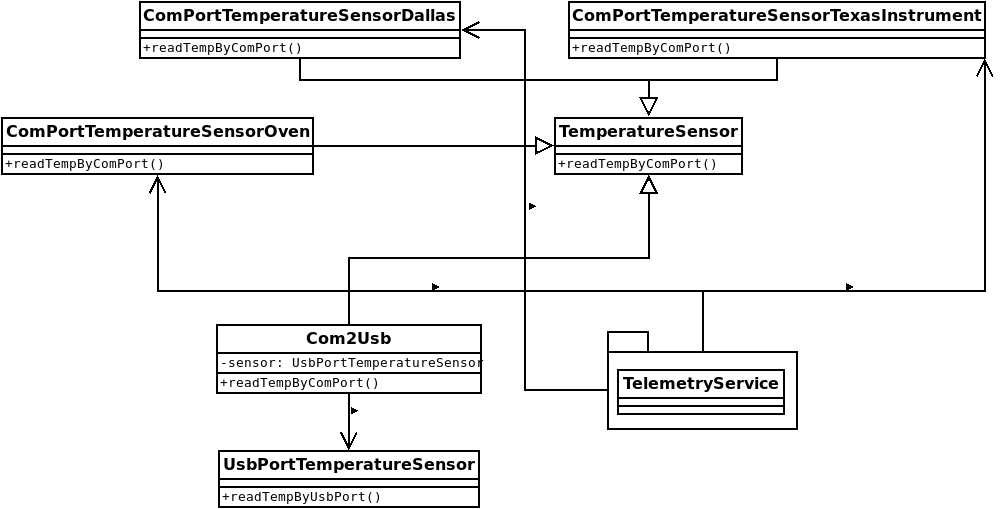
\includegraphics[height=4cm,width=8cm]{adapter-task-resolution1.png}
		\caption{Adapter usage case}
	\end{figure}
\end{frame}

\begin{frame}[fragile]
	\frametitle{Realisation}
	\begin{exampleblock}{Two types of adapters}
		\begin{itemize}
		\item object --- realisation  via composition;
		\item class --- realisation via inheritance.
		\end{itemize}
	\end{exampleblock}
\end{frame}

\begin{frame}[fragile]
	\frametitle{Applicability}
	\begin{exampleblock}{}
		\begin{itemize}
		\item you want to use an existing class, and its interface does not match the one you need.
		\item you want to create a reusable class that cooperates with unrelated or
		unforeseen classes, that is, classes that don't necessarily have compatible interfaces.
		\item (object adapter only) you need to use several existing subclasses, but it's
		unpractical to adapt their interface by subclassing every one. An object adapter
		can adapt the interface of its parent class.
	\end{itemize}
	\end{exampleblock}
\end{frame}

\subsection{Bridge}
\begin{frame}[fragile]
	\frametitle{Intent}
	\begin{exampleblock}{}
	Decouple an abstraction from its implementation so that the two can vary independently
	\end{exampleblock}
\end{frame}
% 
% \begin{frame}[fragile]
% 	\frametitle{Motivation}
% 	\begin{exampleblock}{}
% 	\end{exampleblock}
% \end{frame}
% 
% \begin{frame}[fragile]
% 	\frametitle{Applicability}
% 	\begin{exampleblock}{}
% 		\begin{itemize}
% 		\end{itemize}
% 	\end{exampleblock}
% \end{frame}
% 
% \subsection{}
% \begin{frame}[fragile]
% 	\frametitle{Intent}
% 	\begin{exampleblock}{}
% 	\end{exampleblock}
% 
% 		\begin{figure}
% 			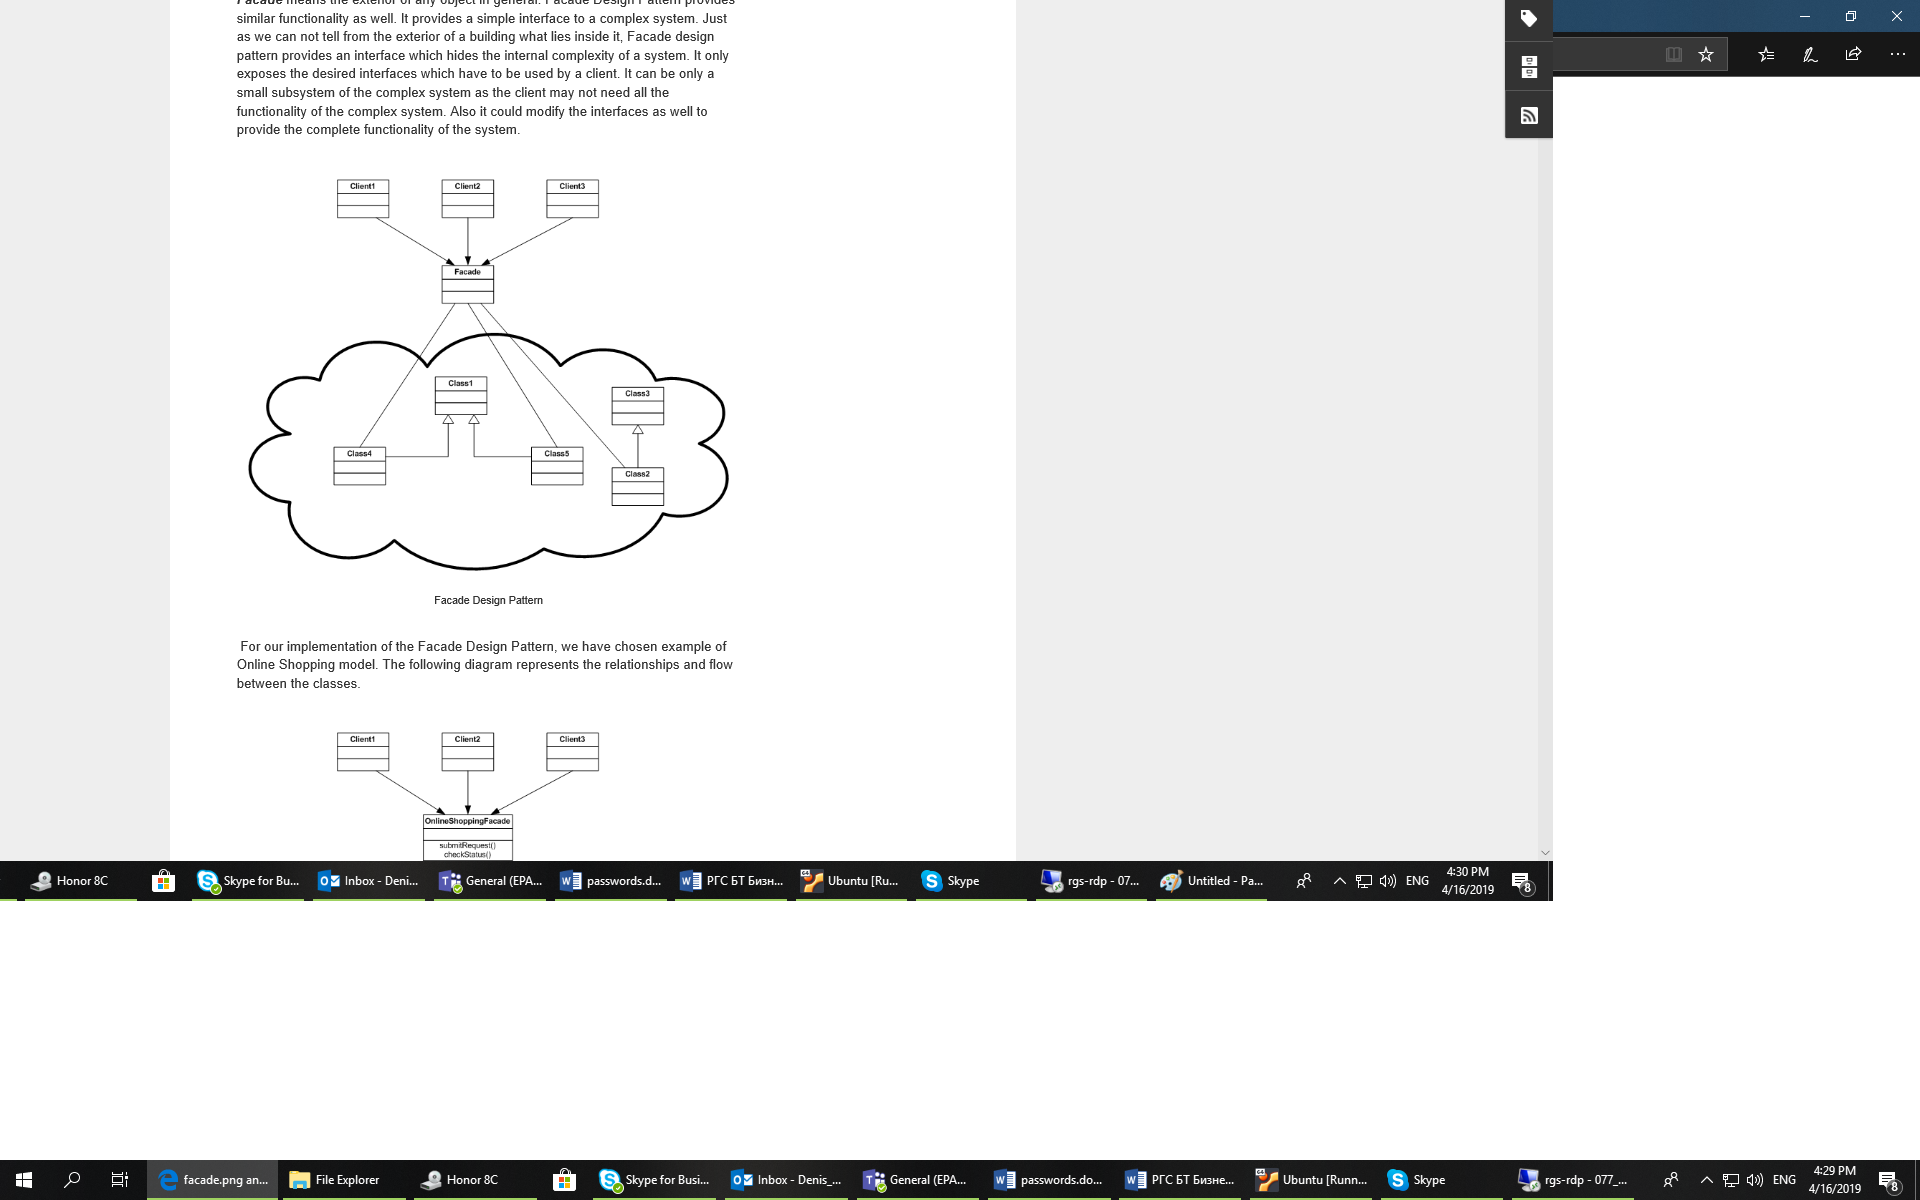
\includegraphics[height=1.2cm,width=6cm]{facade.png}
% 			\caption{Facade UML-diagram}
% 		\end{figure}
% 
% \end{frame}
% 
% \begin{frame}[fragile]
% 	\frametitle{Motivation}
% 	\begin{exampleblock}{}
% 	\end{exampleblock}
% \end{frame}
% 
% \begin{frame}[fragile]
% 	\frametitle{Applicability}
% 	\begin{exampleblock}{}
% 		\begin{itemize}
% 		\end{itemize}
% 	\end{exampleblock}
% \end{frame}


% \subsection{}
% \begin{frame}[fragile]
% 	\frametitle{Intent}
% 	\begin{exampleblock}{}
% 	\end{exampleblock}
% 
% 		\begin{figure}
% 			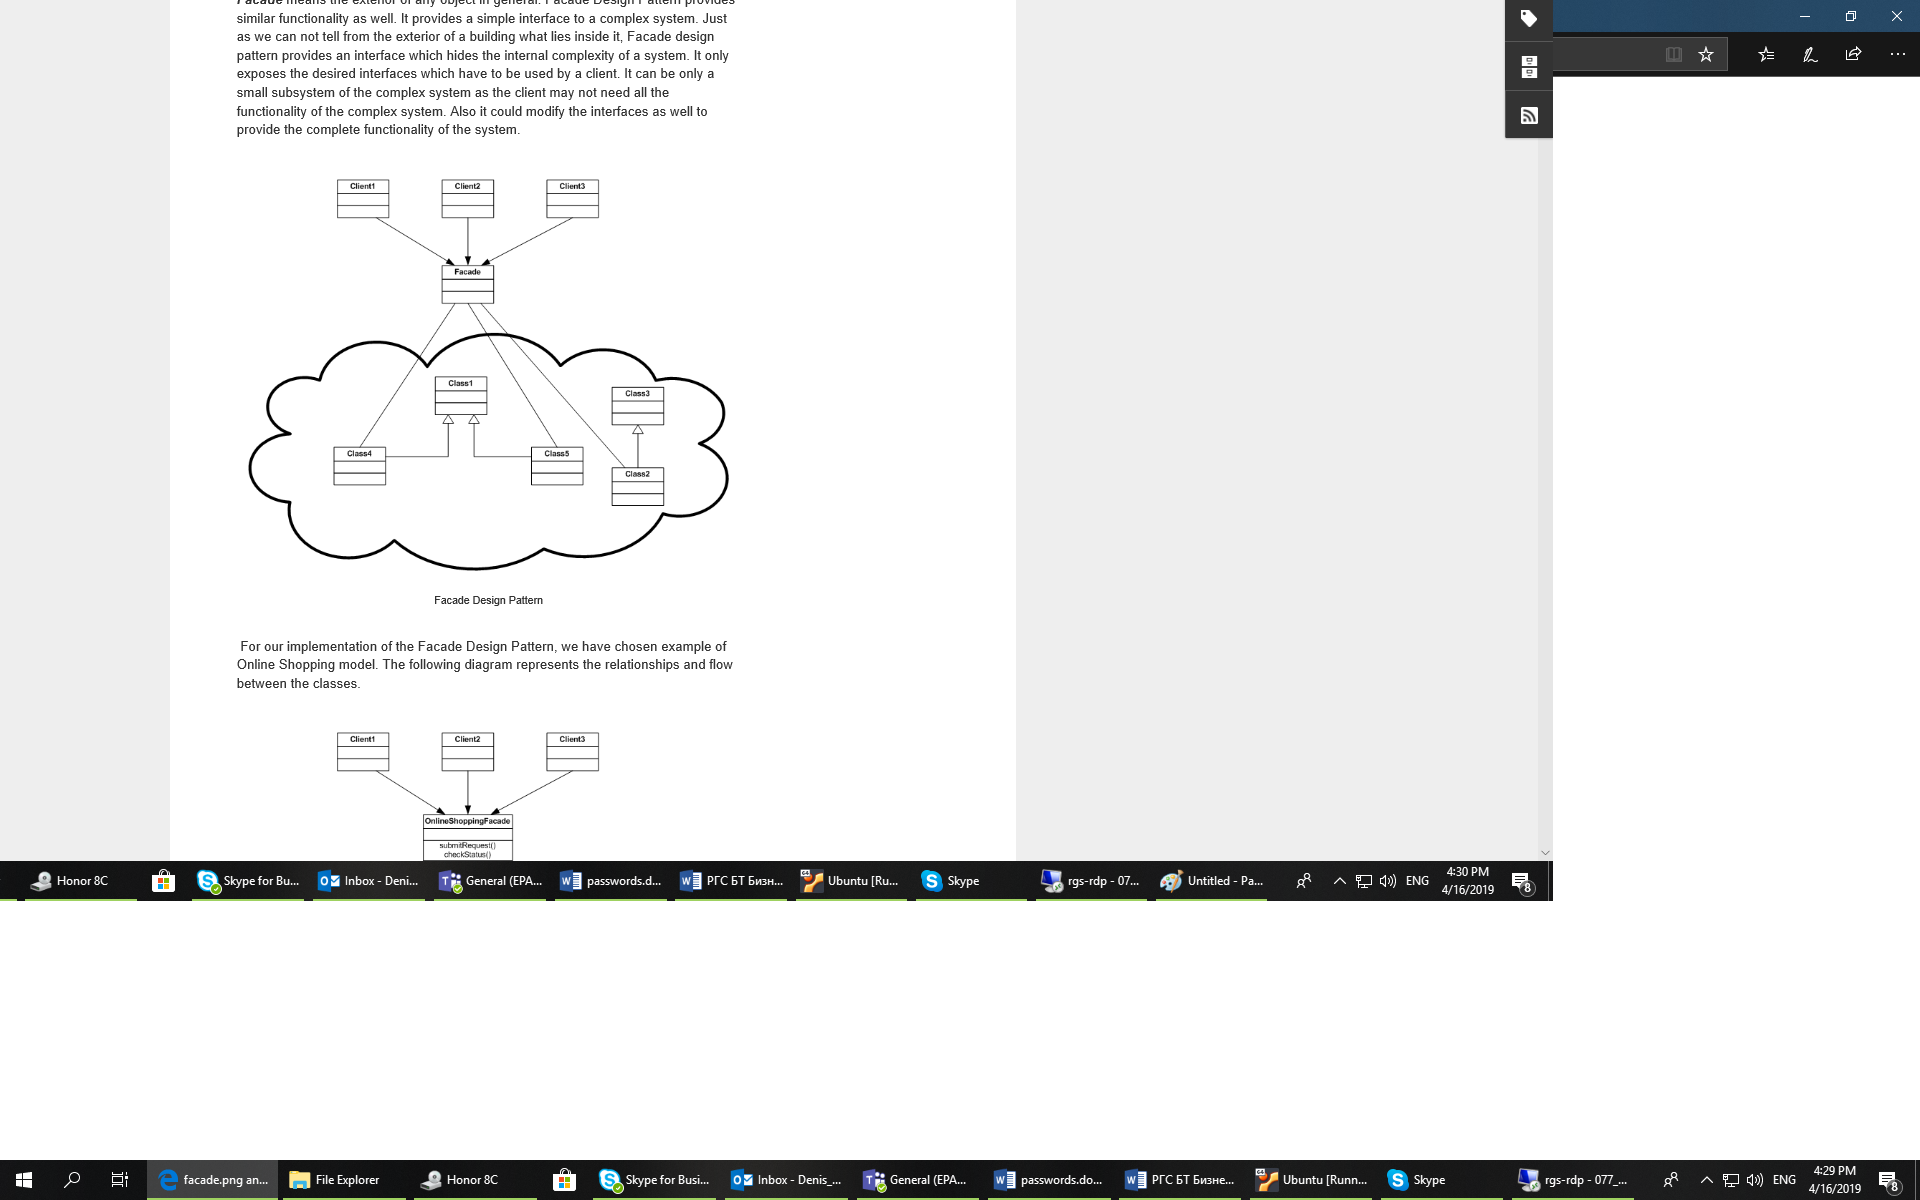
\includegraphics[height=1.2cm,width=6cm]{facade.png}
% 			\caption{Facade UML-diagram}
% 		\end{figure}
% 
% \end{frame}
% 
% \begin{frame}[fragile]
% 	\frametitle{Motivation}
% 	\begin{exampleblock}{}
% 	\end{exampleblock}
% \end{frame}
% 
% \begin{frame}[fragile]
% 	\frametitle{Applicability}
% 	\begin{exampleblock}{}
% 		\begin{itemize}
% 		\end{itemize}
% 	\end{exampleblock}
% \end{frame}


\end{document}

